%!TEX root = ../main.tex
\chapter{Characterizing bottleneck in mobile page load}\label{ch:bottleneck}
As discussed earlier in \S\ref{ch:introduction}, lots of parameters are involved in a page load process.
We also categorized activities involved in a page load, in two main classes: networking activities and computation activities.\\
In this chapter we start off by studying the importance of these two classes and observe how they effect the page load time.
Then, we will look into the critical path and how that would be affected in different situations.

\noindent Characterizing mobile page load times would be our first step towards improving page load performance.

\section{Computation is the bottleneck}

In this section, we show the results of experiments we have run under different network profiles for our set of Web pages, as discussed in \S\ref{sec:parameters}.
We test both desktop and mobile browsers and show the main bottleneck in a page load process.

Our main observations are as follows: 
\begin{itemize}
\item On mobile devices, when analyzing critical path, we observe that in almost all network profiles, ranging from  {\em average lab\_Wifi} to {\em poor lab\_3G}, computation time, rather than networking time, is the dominant factor in the whole page load time .
On contrary, on desktop browsers, networking time takes the majority of the page load time, independent of network profile.
\item Computation still continues to be the bottleneck even when we switch to the new Samsung Galaxy S6 phones, with better computation resources.

\item Computation is still bottleneck on mobile browsers when pages are loaded {\em in-the-wild}. i.e from the original Web server on real WiFi connections rather than in our controlled environment. 
\end{itemize}

\subsection{Page load times}

Figure~\ref{fig:plt_desktop_mobile_mpage} shows the page load times to load pages on desktop browsers, mobile browsers, and to load {\em mpages} on mobile browsers. These are the results of all Web pages and across all network profiles. We can observe that median of page load time on mobile browsers (both original pages and {\em mpages}) is two times greater than that of desktop's in the same network profile.
The difference in tail is much higher. We see later (\S\ref{sec:unrestricted}) that when loading pages on desktop browsers using Ethernet connection, the difference in page load time between mobile and desktop browsers is even higher.

\begin{figure}[!htb]
\centering{
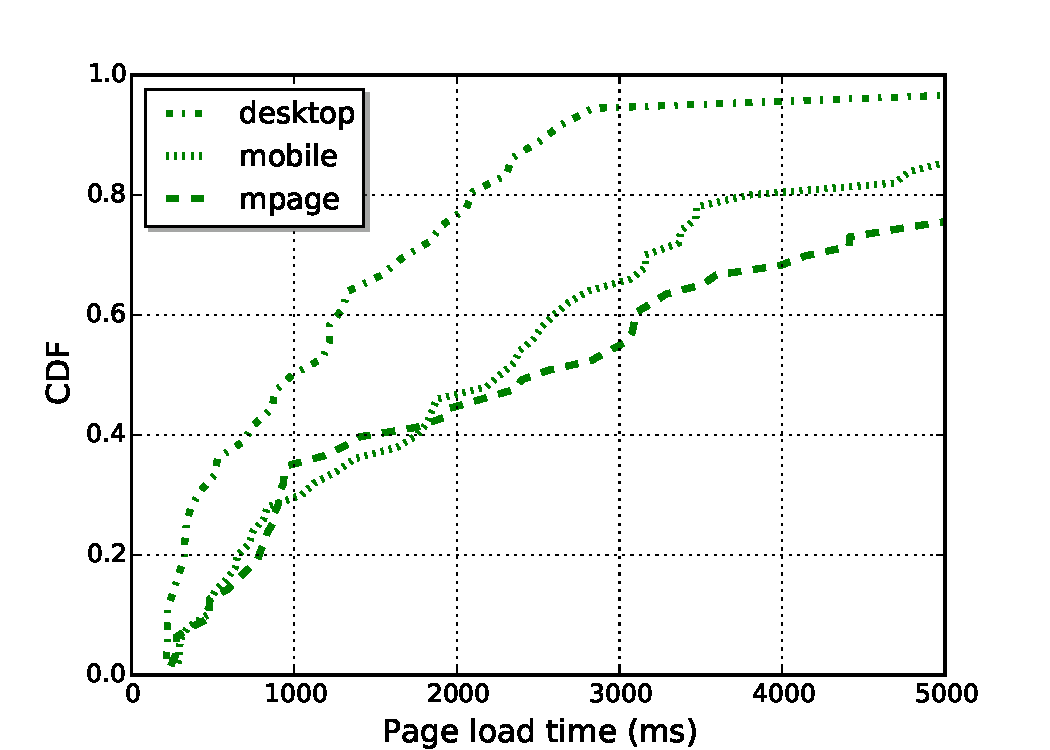
\includegraphics[scale=0.5]{./figures/plt/plt_desktop_mobile_mobileversion.pdf}
\caption{Comparing the page load times between loading original pages on mobile browser vs desktop browser, and loading {\em mpages} on the mobile browser.   }
\label{fig:plt_desktop_mobile_mpage}
}
\end{figure}

\noindent Although {\em mpages} are smaller versions of the original pages, we do not see a significant difference between page load times when loading original pages and {\em mpages} on mobile. Reducing object sizes, would directly affect the download time for those objects but does not necessarily reduce the computation requirement. %proportionally.

\subsection{Bottleneck in mobile vs desktop browsers}
In order to pinpoint the bottleneck in a page load process, we load the same set of Web pages on desktop ad the mobile browsers, under the same network conditions.
Figure~\ref{fig:comp_net_fraction_average} shows the fraction of computation activities on the critical path and the fraction of network activities on the critical path for desktop browsers. Figures~\ref{fig:non-mobile-b20-d50} and~\ref{fig:non-mobile-b5-d50} show that downloading objects takes 60\% of the total delay on the critical path, while the computation activities is responsible for only  40\% of the total delay on the critical path. This relation holds for different network profiles.

\begin{figure}[!htb]
    \begin{subfigure}{0.48\textwidth}
        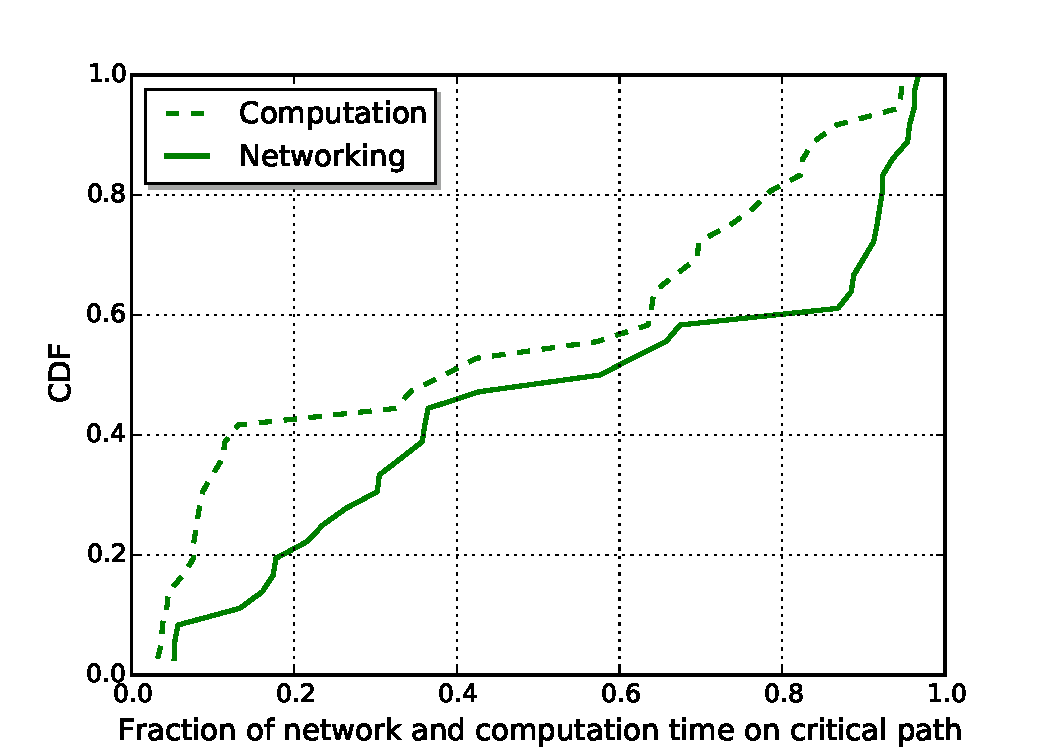
\includegraphics[width=1\linewidth]{./figures/computation/desktop-b20-d50.pdf}
        \caption{Desktop, Average lab\_Wifi}
        \label{fig:non-mobile-b20-d50}
    \end{subfigure}%
    \begin{subfigure}{0.48\textwidth}
        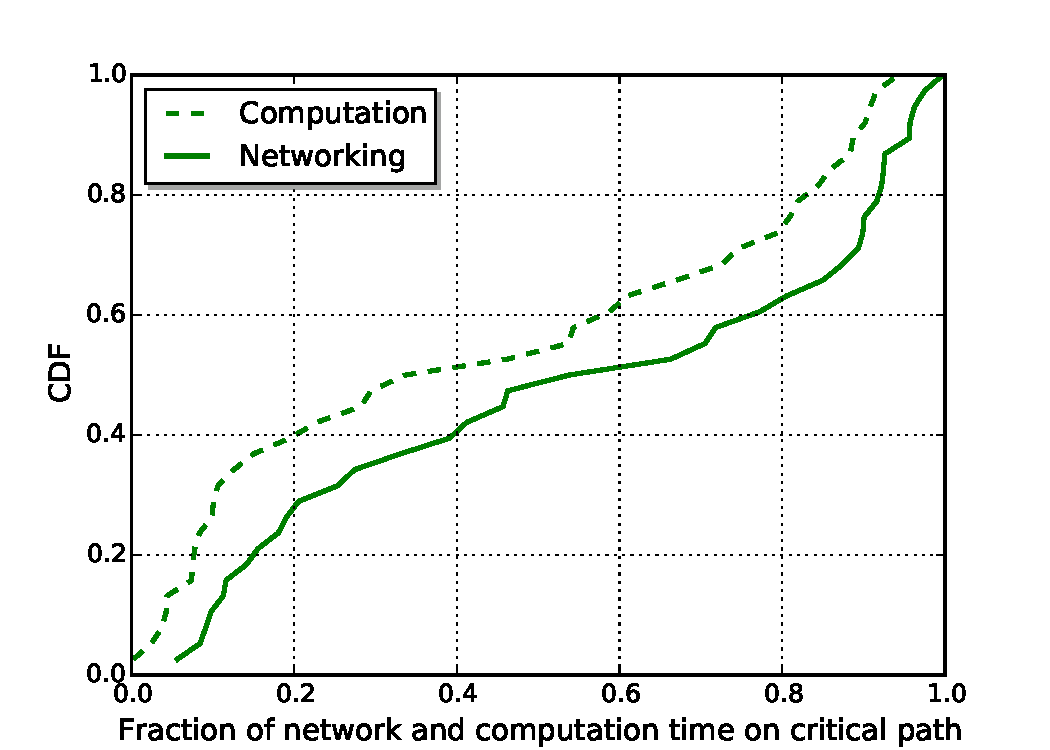
\includegraphics[width=1\linewidth]{./figures/computation/desktop-b5-d50.pdf}
        \caption{Desktop, Average lab\_4G}
        \label{fig:non-mobile-b5-d50}
    \end{subfigure}
   \begin{subfigure}{0.48\textwidth}
        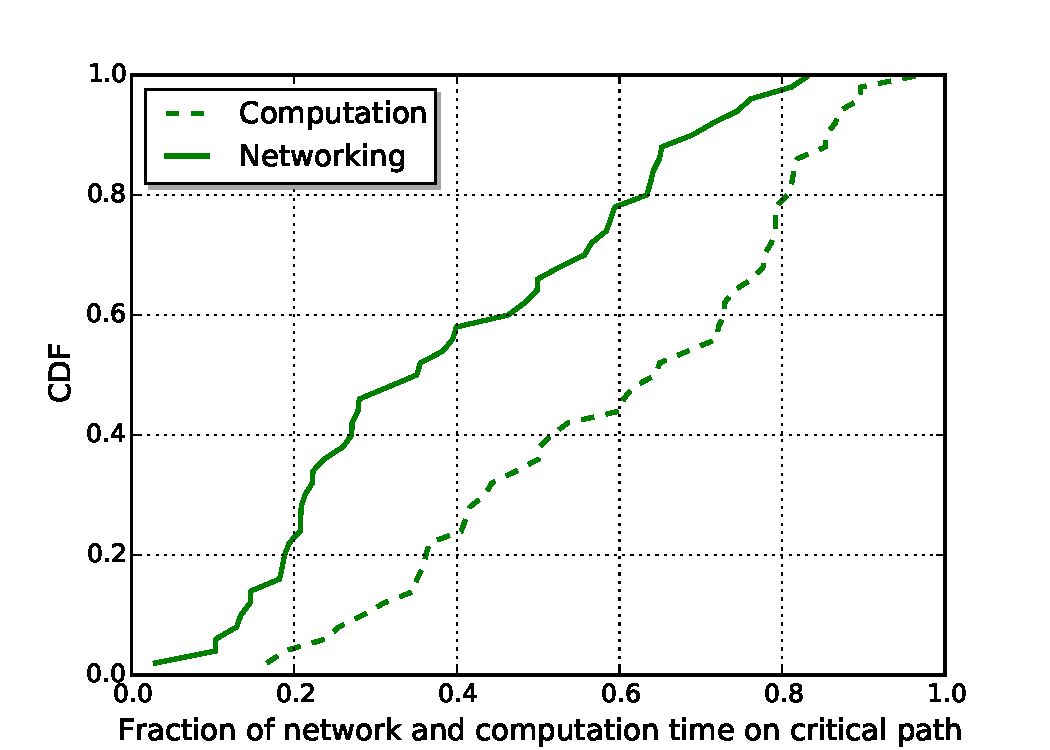
\includegraphics[width=1\linewidth]{./figures/computation/mobile-b20-d50.pdf}
        \caption{Mobile, Average lab\_Wifi}
        \label{fig:mobile-b20-d50}
    \end{subfigure}%
    \begin{subfigure}{0.48\textwidth}
    \centering
        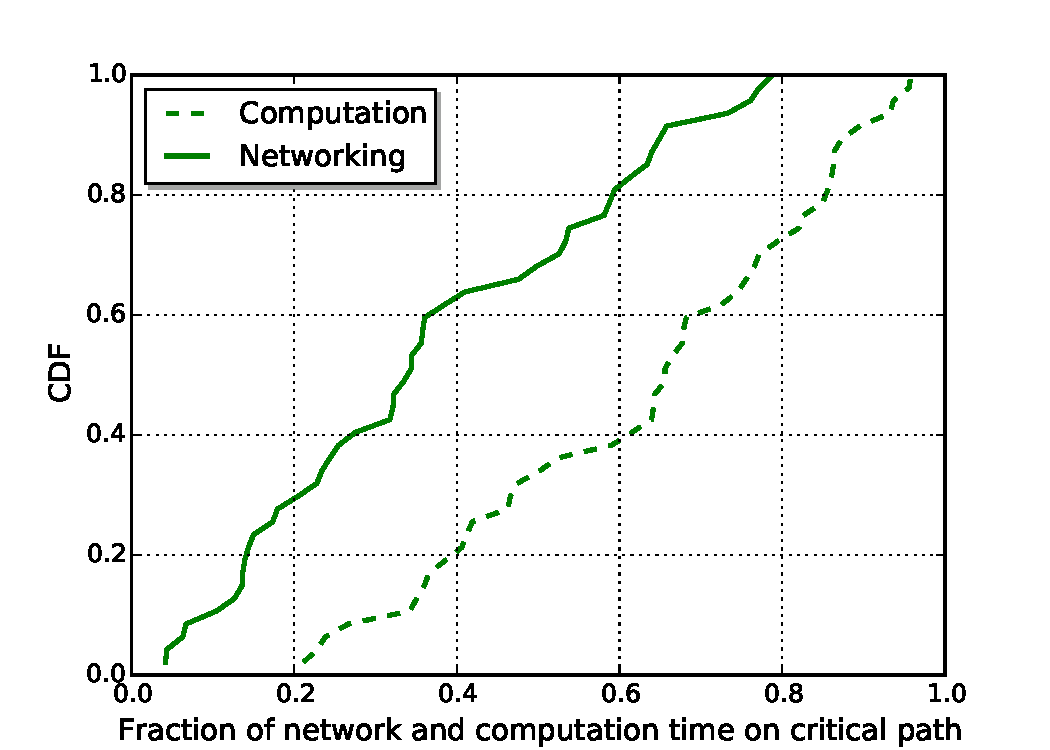
\includegraphics[width=1\linewidth]{./figures/computation/mobile-b5-d50.pdf}
        \caption{Mobile, Average lab\_4G}
        \label{fig:mobile-b5-d50}
    \end{subfigure}
      \caption{Average Wireless Connectivity: Fraction of network and computation time on critical path. Under average connectivity, computation is the main bottleneck for mobile browsers. }
    \label{fig:comp_net_fraction_average}
   \end{figure}
   
\noindent However, for mobile browsers computation time versus network activities time on the critical path  is different. Figure~\ref{fig:mobile-b20-d50} and~\ref{fig:mobile-b5-d50} shows that on both the average lab\_Wifi and the average lab\_4G networks, the bottleneck is the computation activities when loading a page on mobile browsers. Computation accounts for over 60\% of the page load time on the critical path in the median case when loading pages on mobile browsers. The results for the lab\_3G network is quantitatively similar (not shown here).

\noindent Figure~\ref{fig:comp_net_fraction_poor} shows the same bottleneck analysis but when the wireless network is of poor quality with longer round trip times of 150ms. Surprisingly, even when the network is poor, Figure~\ref{fig:mobile-b20-d150} shows that computation remains a bottleneck for page load on poor lab\_WiFi, accounting for 55\% of the page load time in the median case. It is only in the poor lab\_4G environment that the network becomes the bottleneck when loading pages on the mobile browser. On the other hand, on desktop browsers, poor wireless condition only makes the network bottleneck even more pronounced (Figures~\ref{fig:non-mobile-b20-d150} and~\ref{fig:non-mobile-b5-d150}).
\begin{figure}[!htb]
    \begin{subfigure}{0.48\textwidth}
        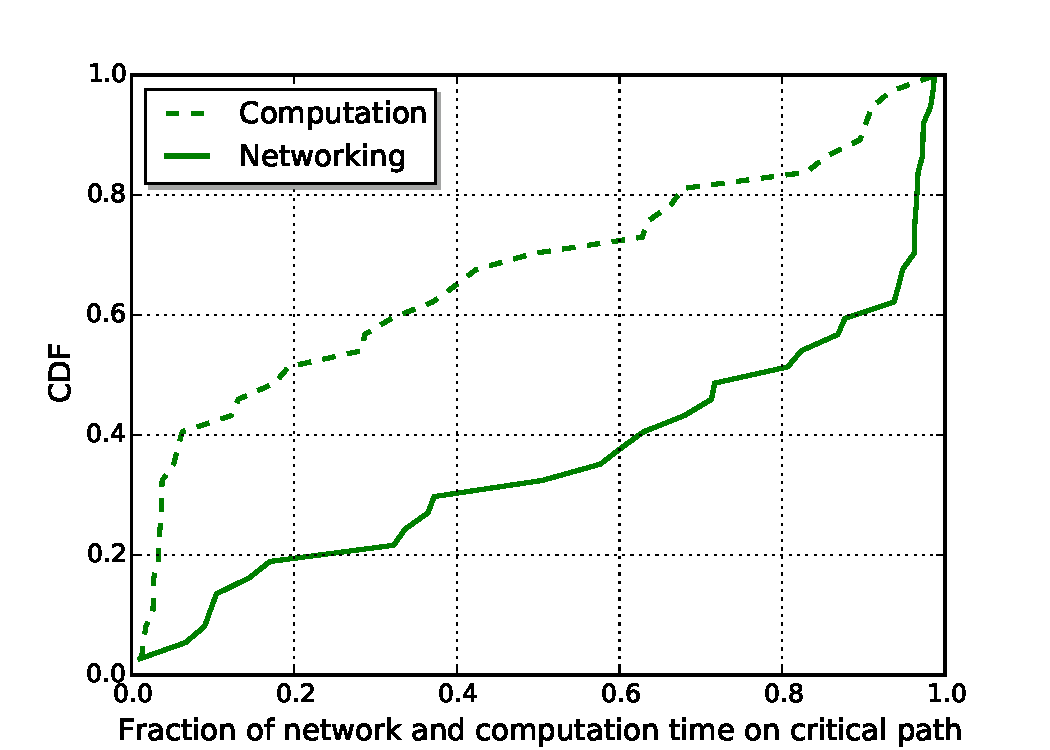
\includegraphics[width=1\linewidth]{./figures/computation/poor/desktop-b20-d150.pdf}
        \caption{Desktop browser, Poor lab\_Wifi}
        \label{fig:non-mobile-b20-d150}
    \end{subfigure}%
    \begin{subfigure}{0.48\textwidth}
        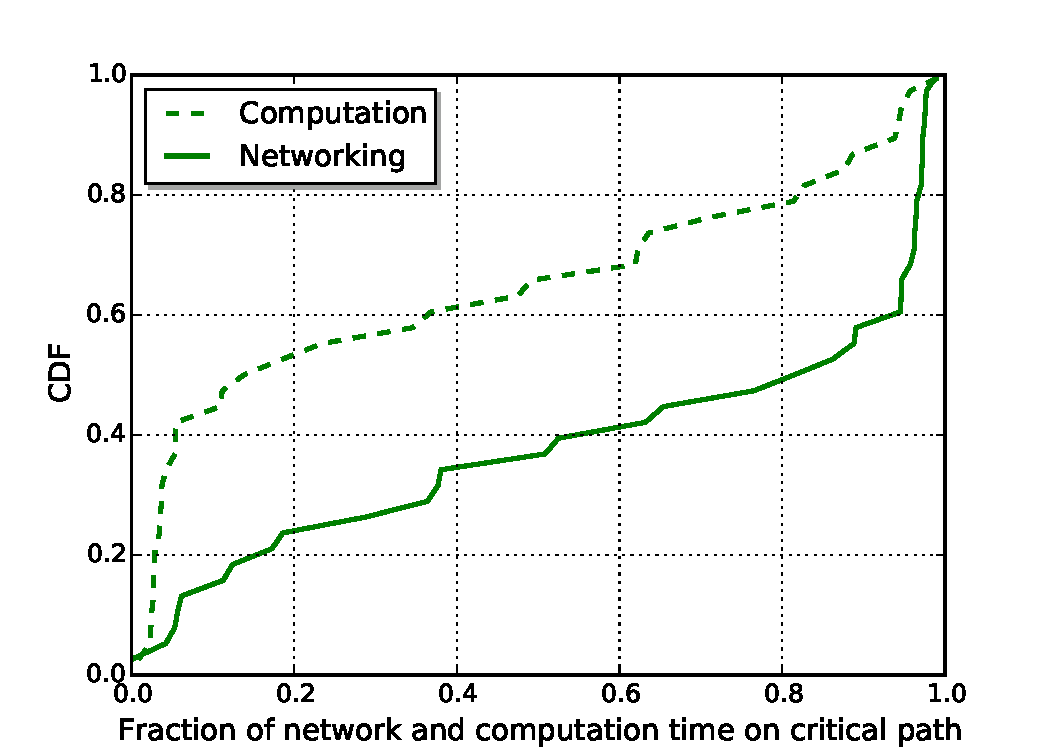
\includegraphics[width=1\linewidth]{./figures/computation/poor/desktop-b5-d150.pdf}
        \caption{Desktop browser, Poor lab\_4G}
        \label{fig:non-mobile-b5-d150}
    \end{subfigure}
   \begin{subfigure}{0.48\textwidth}
        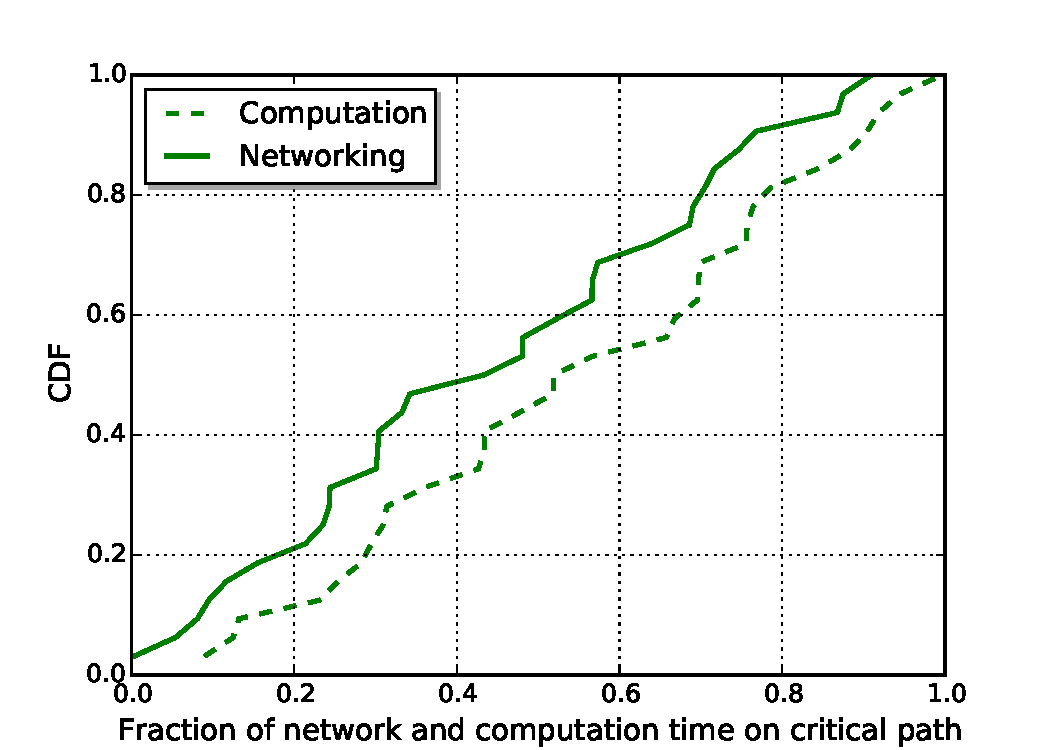
\includegraphics[width=1\linewidth]{./figures/computation/poor/mobile-b20-d150.pdf}
        \caption{Mobile browser, Poor lab\_Wifi}
        \label{fig:mobile-b20-d150}
    \end{subfigure}%
    \begin{subfigure}{0.48\textwidth}
    \centering
        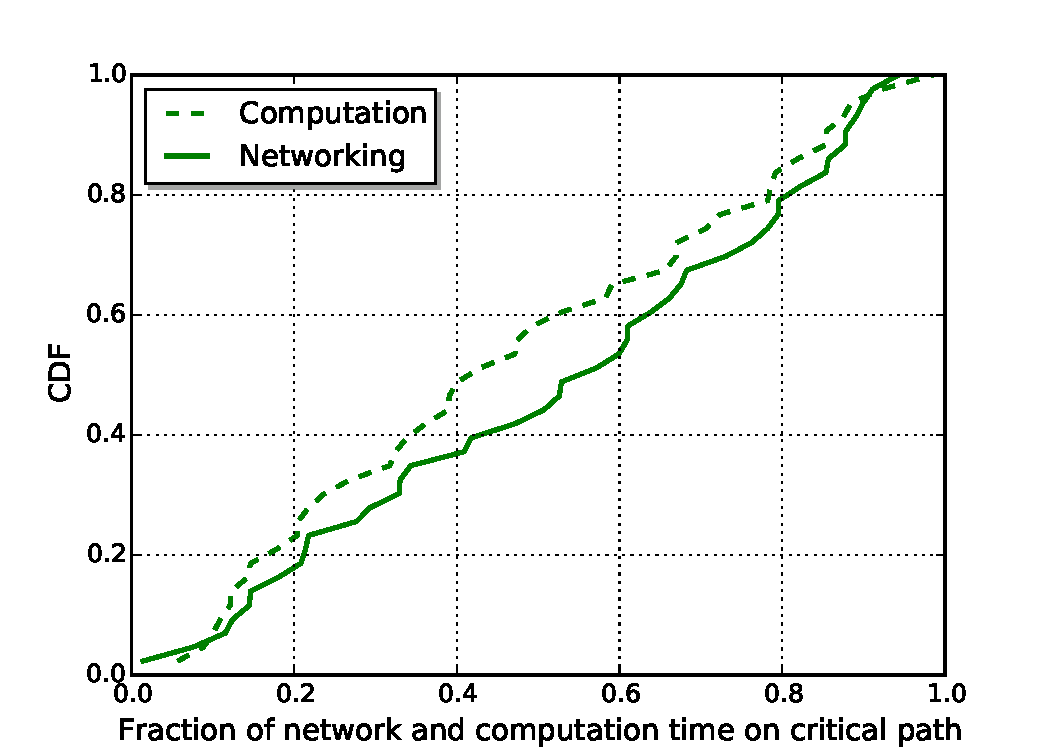
\includegraphics[width=1\linewidth]{./figures/computation/poor/mobile-b5-d150.pdf}
        \caption{Mobile browser, Poor lab\_4G}
        \label{fig:mobile-b5-d150}
    \end{subfigure}
      \caption{Poor Wireless Connectivity: Fraction of network and computation time on critical path. Even under poor network connectivity, computation is the bottleneck for mobile browsers. In contrast, under poor connectivity, network becomes even more of a bottleneck for desktop browsers.}
    \label{fig:comp_net_fraction_poor}
   \end{figure}


\subsection{Bottleneck when loading mpages}
Figure~\ref{fig:comp_network_mpage} shows that when loading {\em mpages} on the mobile browsers, computation is once again the bottleneck. In the median case, more than 60\% of the critical path is spent on computational activities in the median case.
\begin{figure}[!htb]
\centering{
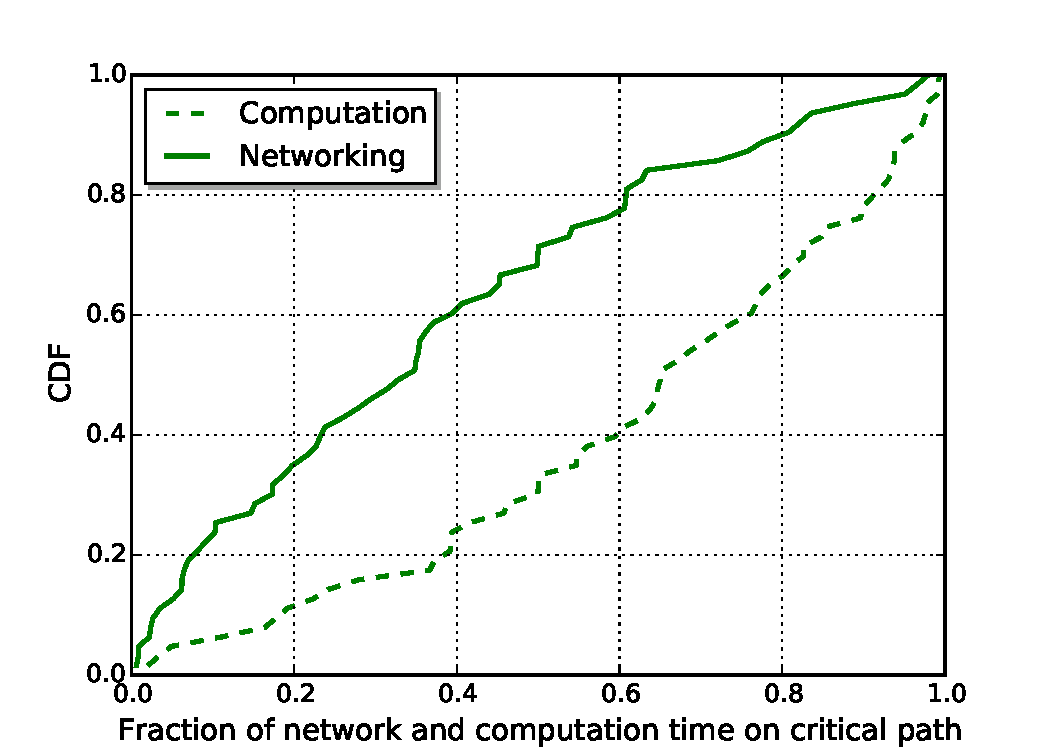
\includegraphics[scale=0.5]{./figures/computation/mobileversion_wifi_b20_d50.pdf}
\caption{Loading {\em mpages} on lab\_Wifi: The fraction of network and computation on critical path. }
\label{fig:comp_network_mpage}
}
\end{figure}


\subsection{Experiments on Samsung Galaxy S6}
 We ran the controlled page load experiments again on Samsung Galaxy S6, which has a 2100MHz CPU and octo-core, compared to the quad-core, 1700MHz Samsung S4 phones. Figure~\ref{fig:plt_s6_b5_d50} shows that the page load time on S6 is not much different compared to the page load time on S4. 

\noindent Interestingly, Figure~\ref{fig:comp-net-s6-b5-d50} shows that the computation is still a bottleneck for the page load, even under a better CPU specification. This results suggests that browsers are not utilizing the additional CPU capacity in newer phones effectively. 

\subsection{Experiments "in-the-wild"}
\label{sec:unrestricted}

\begin{figure}[!htb]
  \begin{subfigure}{0.48\textwidth}
     \centering{
        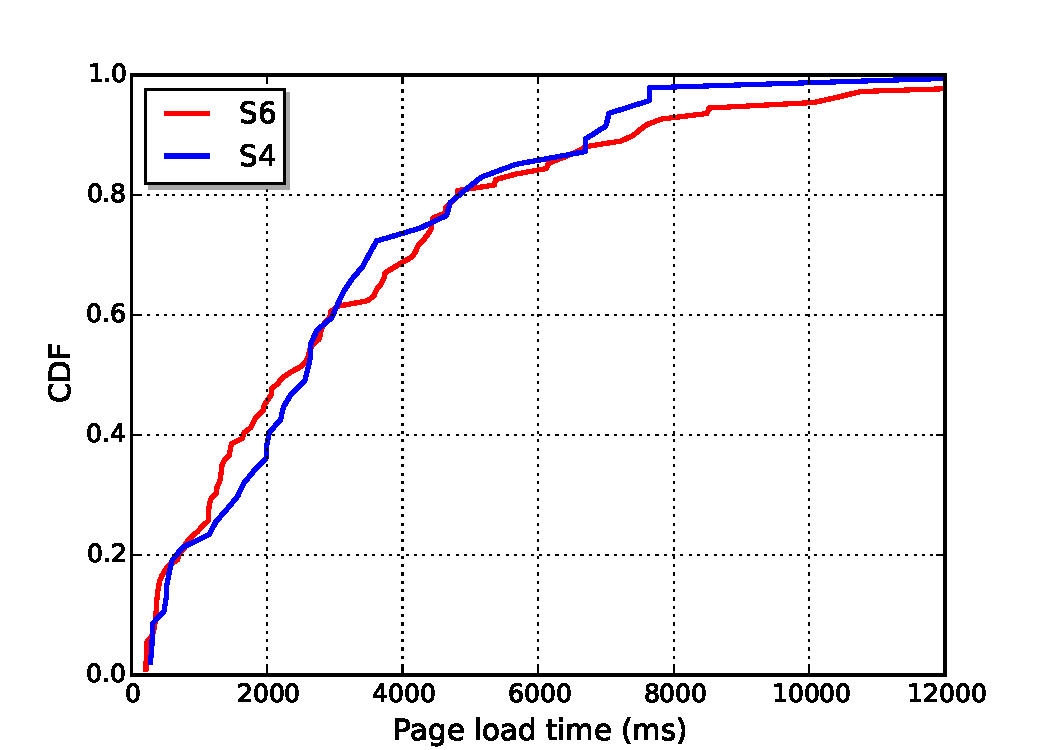
\includegraphics[width=1\linewidth]{./figures/s6/plt_s4_s6_mobile_b5_d50.pdf}
        \caption{PLTs when loading web pages on Samsung Galaxy S4 and S6 phones. The pages were loaded in the average lab\_4G network. }
        \label{fig:plt_s6_b5_d50}
    }
 \end{subfigure} \hspace{0.1in}%
\begin{subfigure}{0.48\textwidth}
            \centering{
        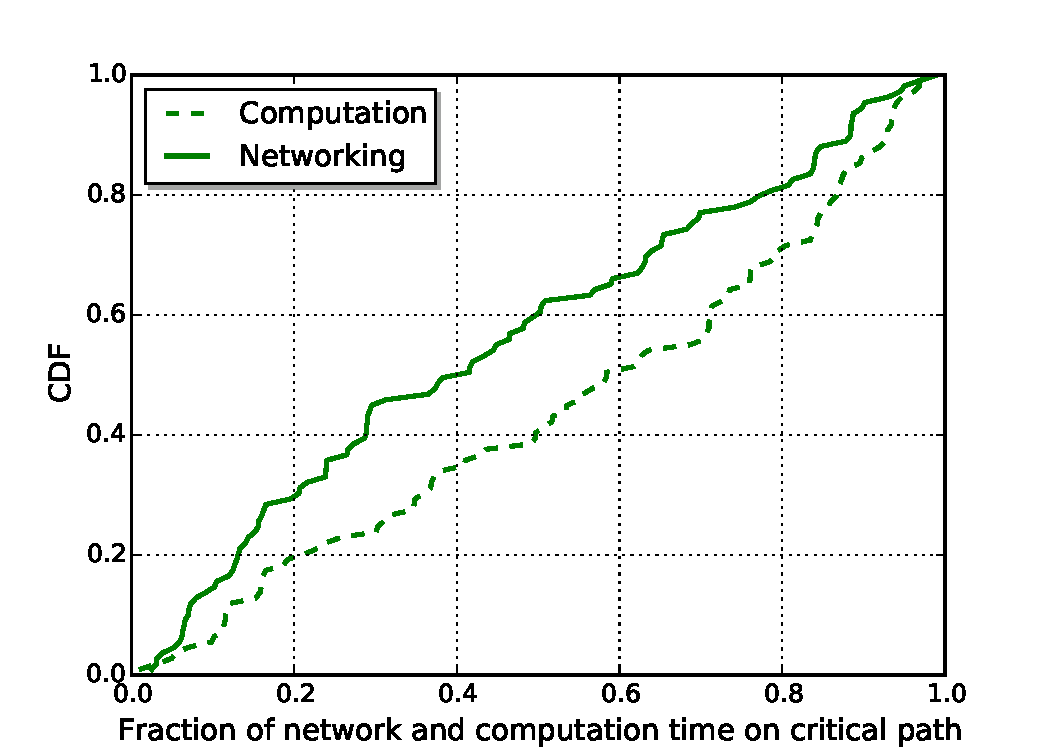
\includegraphics[width=1\linewidth]{./figures/s6/mobile_s6_b5-d50.pdf}
        \caption{Computation vs Networking on critical path  when loading pages in Samsung Galaxy S6 phones under average lab\_4G network conditions.}
        \label{fig:comp-net-s6-b5-d50}
        }
        \end{subfigure}
        \caption{Results from experiments on Samsung Galaxy S6}
        \label{fig:s6}
  \end{figure}


\noindent Finally, we load web pages on desktop and mobile browsers outside of our experimental testbed.  The web pages are fetched from the original Web server. The desktop browser uses the campus Ethernet connection (bandwidth 250Mbps), while the mobile browser uses the campus WiFi connection (bandwidth 30Mbps). The goal of this experiment is to study if the observations we make in the controlled setting also hold true in general. Note that as there are variances in networking parameters when running experiments {\em in-the-wild}, we cannot make generalizations in this case.

\begin{figure}[!htb]
\begin{minipage}[b]{.48\textwidth}
  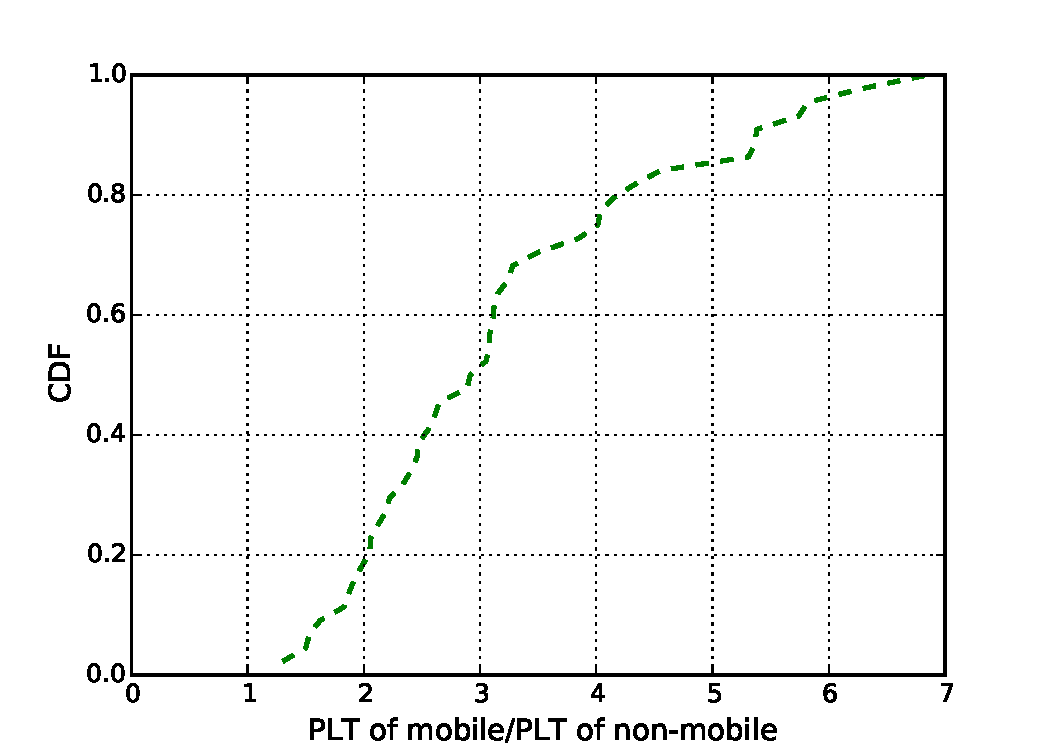
\includegraphics[width=\linewidth]{./figures/uncontrolled/mobile_desktop_plt_ratio_uncontrolled.pdf}
  \captionof{figure}{PLT difference between loading pages on mobile and desktop in-the-wild.}
  \label{fig:plt_uncontrolled_mobile_desktop}
\end{minipage}%
\hspace{0.5cm}
\begin{minipage}[b]{.48\textwidth}
  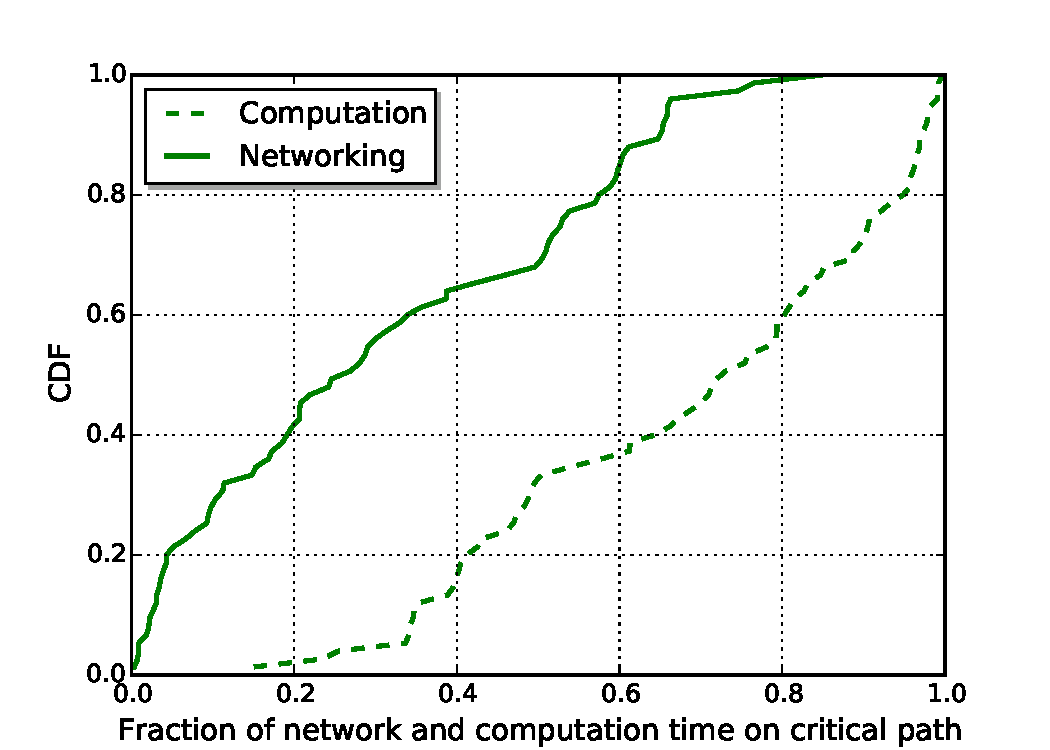
\includegraphics[width=\linewidth]{./figures/uncontrolled/mobile_uncontrolled.pdf}
  \captionof{figure}{Mobile browser in the wild: computation vs networking on critical path.}
  \label{fig:network_comp_uncontrolled_mobile}
\end{minipage}
\end{figure}

\noindent Figure~\ref{fig:plt_uncontrolled_mobile_desktop} shows the ratio of the time to load the page on mobile browsers and desktop browsers. The difference in page load time is even higher compared to the experiment in the controlled setting (Figure~\ref{fig:plt_desktop_mobile_mpage}). Loading pages on the mobile browser is three times as slow as the desktop in the median case. This is largely because of the difference in network speeds between Ethernet and WiFi.

\noindent Surprisingly, Figure~\ref{fig:network_comp_uncontrolled_mobile} shows that, similar to the controlled setting, the bottleneck in mobile browser remains computation.
%
%critical path analysis
%
\section{Critical path analysis}

Next, we study critical path in loading Web pages on mobile and desktop browsers. Summary of our observations are as follows:
\begin{itemize} 

\item Although number of Javascripts, CSS, images, and HTML evaluations seems to be similar on critical path, when the same web pages are loaded on the same network profiles, but objects are not exactly the same. In other words, activity type distribution remains similar, while they are different activities.

\item Each computation activity on the critical path, takes 4 times longer when is run on mobile browser compared to the desktop browser.

\end{itemize}
\subsection{Object downloads}

Figure~\ref{fig:numbytesall} depicts the total number of bytes downloaded when loading the original page and loading the {\em mpage} on a mobile browser in all network profiles. Even though {\em mpages} are designed to be smaller, we find that for 60\% of the pages, the total data downloaded remains the same. But for 30\% of the pages, the difference in size is over 60\%. The results suggests that {\em mpages} significantly reduce the size of a small number of pages, but for a large fraction of pages, there is not much difference between {\em mpages} and the original page.

Figure~\ref{fig:numbytescp} shows the bytes downloaded on the critical path for original page and {\em mpage}. Recall that only objects loaded in the critical path contribute to the page load time; other objects are loaded in parallel. Here we find that {\em mpages} reduce the number of objects loaded in the critical path for over 40\% of the pages. In other words, {\em mpages} does reduce the network latency on the critical path.

However, the page load time does not reduce significantly when loading {\em mpages} compared to the original pages (see Figure~\ref{fig:plt_desktop_mobile_mpage}). This is because the computation is the bottleneck when loading {\em mpages} on the mobile browser, as shown in Figure~\ref{fig:comp_network_mpage}. In a separate experiment (not shown here), we find that loading {\em mpages} does not reduce the computation time on the critical path. In fact, the computation time is slightly worse. 

\subsection{Similarity metric}

We load the same pages on mobile and desktop browsers, under the same network environments. This lets us compare the critical path of the page load on mobile and desktop browsers. The critical path consists of a series of activities such as loading an object, evaluating a Javascript, etc. In addition, each activity is associated with a unique URL corresponding to the activity. For example, the URL of the object to be loaded, or the URL of the Javascript to be evaluated.


\begin{figure}[!htb]
\begin{minipage}[b]{.48\textwidth}
  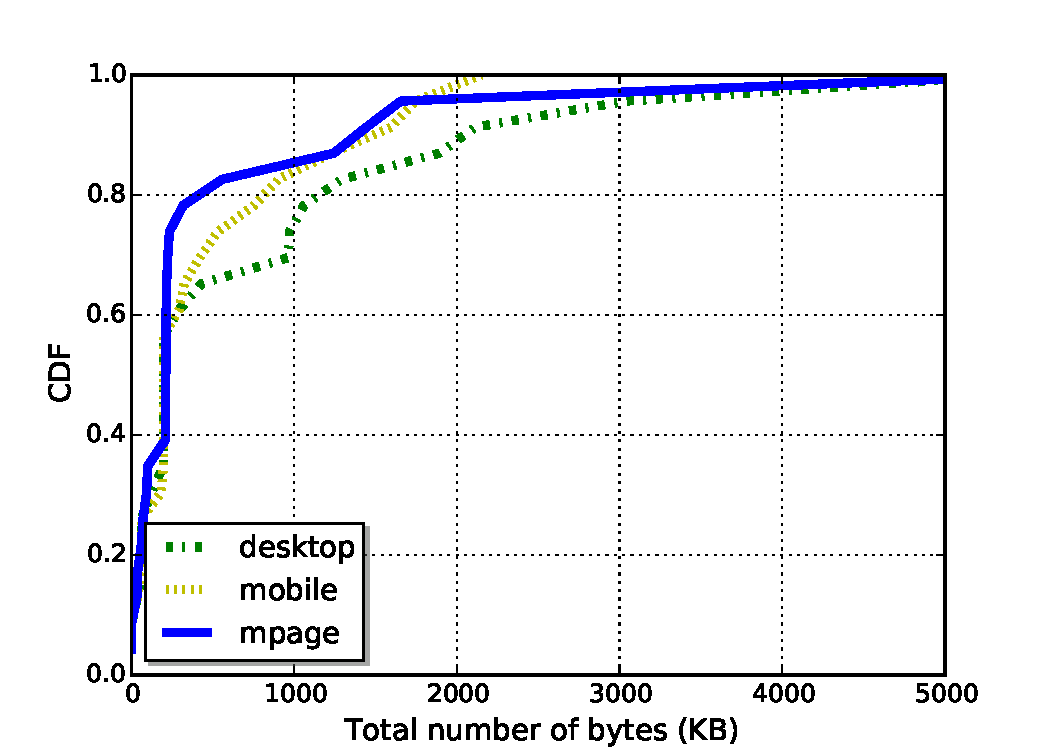
\includegraphics[width=\linewidth]{./figures/criticalpath/num_bytes_all.pdf}
  \captionof{figure}{Number of total bytes downloaded for{ \em mobile} and{ \em mpage} }
  \label{fig:numbytesall}
\end{minipage}%
\hspace{0.5cm}
\begin{minipage}[b]{.48\textwidth}
  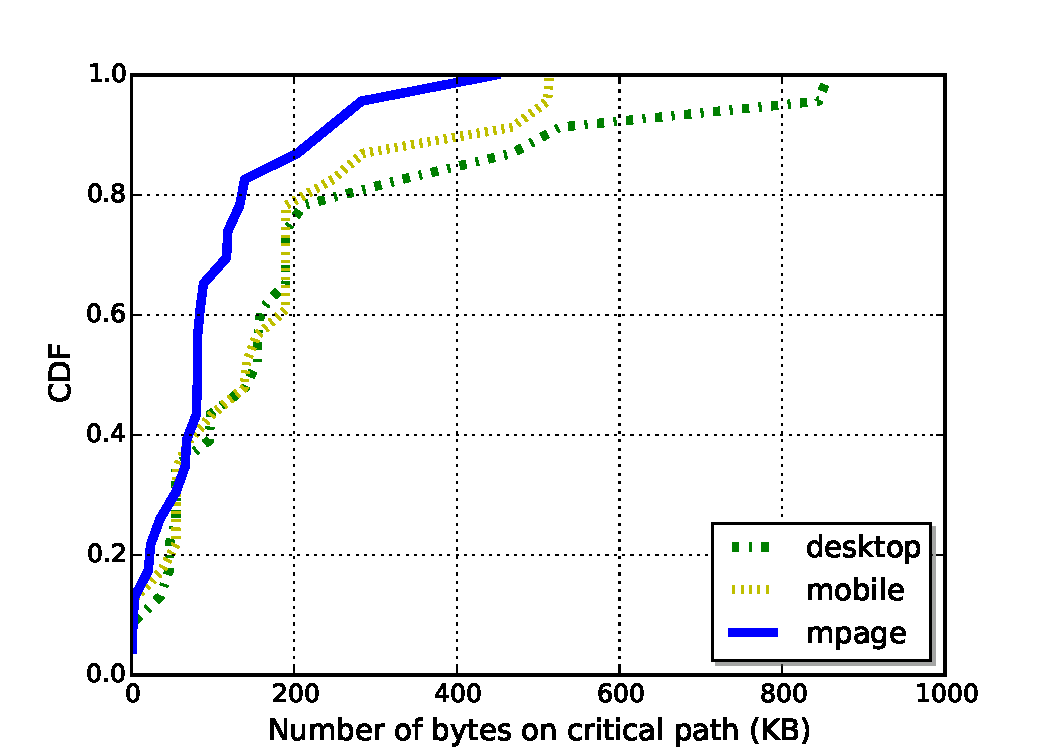
\includegraphics[width=\linewidth]{./figures/criticalpath/num_bytes_cp.pdf}
  \captionof{figure}{Number of bytes download on critical path for{ \em mobile} and{ \em mpage}}
  \label{fig:numbytescp}
\end{minipage}
\end{figure}

\noindent We define similarity metric as follows: the fraction of time the same <URL, activity> pair occurs  both on the critical path of the mobile page load and the critical path of the desktop page load. If the number of elements on the critical path are not equal, we pad the smaller critical path with null activities.

\noindent Figure~\ref{fig:similarity} shows the similarity metric across all network profiles. Even when the same page is being loaded under the same network profile, the critical path is identical only for 20\% of pages. For another 20\% of the pages, only 50\% of the critical path is similar. This result has big implications for optimization. It shows that optimizing a specific object, such as making a specific Javascript object smaller, may not have the same effect on mobile browsers as they would desktop browsers.

\begin{figure}[!htb]
  \centering
    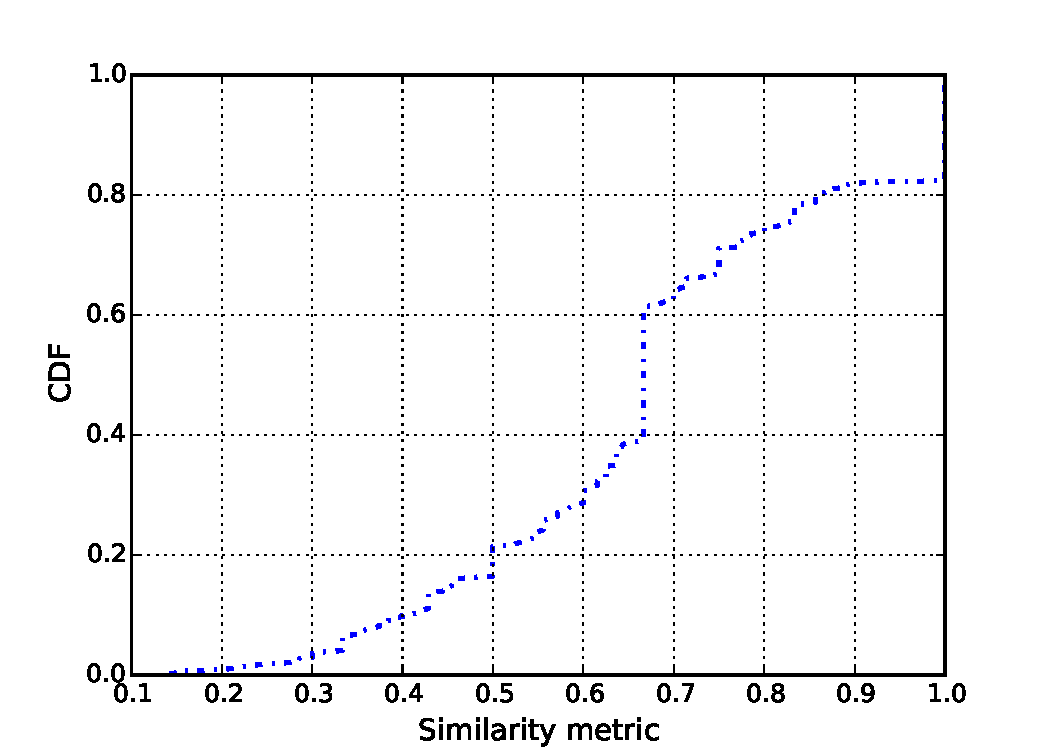
\includegraphics[width=0.5 \textwidth]{./figures/criticalpath/similarity.pdf}
  \caption{Similarity metric: the fraction of time the same <URL, activity> pair occur on the critical path of both mobile and desktop page load. }
  \label{fig:similarity}
\end{figure}

\noindent Next, we relax the definition of similarity and look at the percentage of time the same activity occur on the critical paths. For example, if there two Javascript activities on both critical paths, but the URLs corresponding to the Javascript are different, we still define the two activities as being similar.  For this definition of similarity, we also include the experiments where we loaded the mobile version of the pages.

\noindent Figure \ref{fig:bar_plot_percentage} shows the percentage of each activity on the critical path across all pages and network profiles. In terms of the activities, we see that the critical path is very similar. In other words, for every page, the activities on the critical path in terms of Javascript evaluation, HTML parsing etc are similar on desktop and mobile browsers. But the critical paths differ in terms of, for example, which Javascript is being evaluated. One of the implications of this result is that, optimizations that target a class of activities, such as reducing the time to download all Javascript objects, are likely to provide benefits across mobile and desktop browsers.

\begin{figure}[!htb]
  \centering
    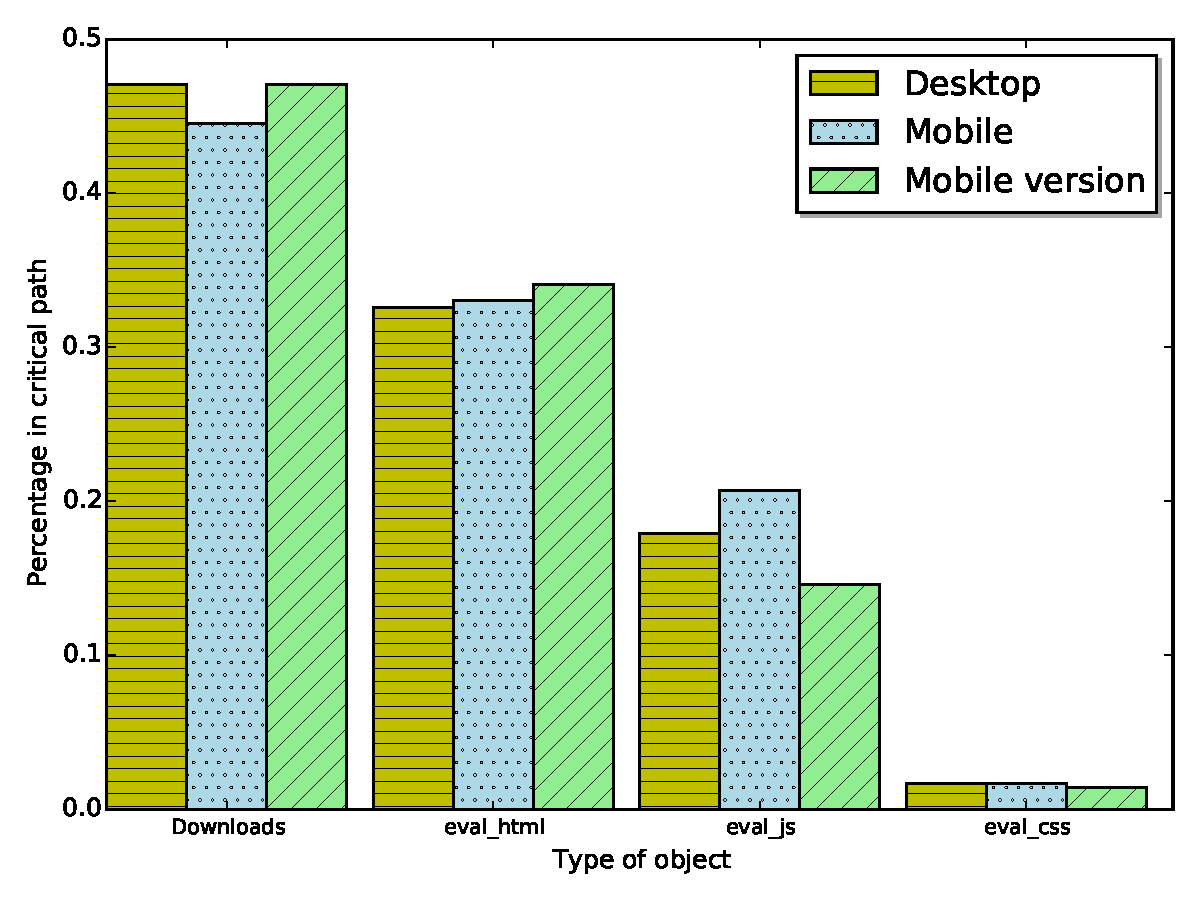
\includegraphics[width=0.5\textwidth]{./figures/criticalpath/bar_plot_percentage.pdf}
  \caption{Fraction of different activities on the critical path. }
  \label{fig:bar_plot_percentage}
\end{figure}

\subsection{Latency for each activity on the critical path}

Finally, we measure the difference in latencies when performing the same activity on the mobile versus the desktop browser.  To this end, we identify each activity on the critical path of either the desktop load or the mobile load. We then compare the latency of this activity when loading on the desktop versus loading on the mobile browser. Since we load the exact same page, an activity such as loading a specific Javascript  will have to be performed both on the desktop load and the mobile load.

\noindent Figure~\ref{fig:bar_plot_percentage} shows the time take of each activity to be performed on the mobile versus the desktop browser. Each computation activity takes over 4 times longer to perform on the mobile browser versus the desktop browser. This is the core reason for the computational bottleneck on mobile browsers. For 50\% of the web pages, it takes slightly longer to perform network activities on the mobile browser compared to desktop browser. This can possibly be because of a less optimized network stack on the mobile browser compared to desktop browser.

\begin{figure}[!htb]
  \centering
    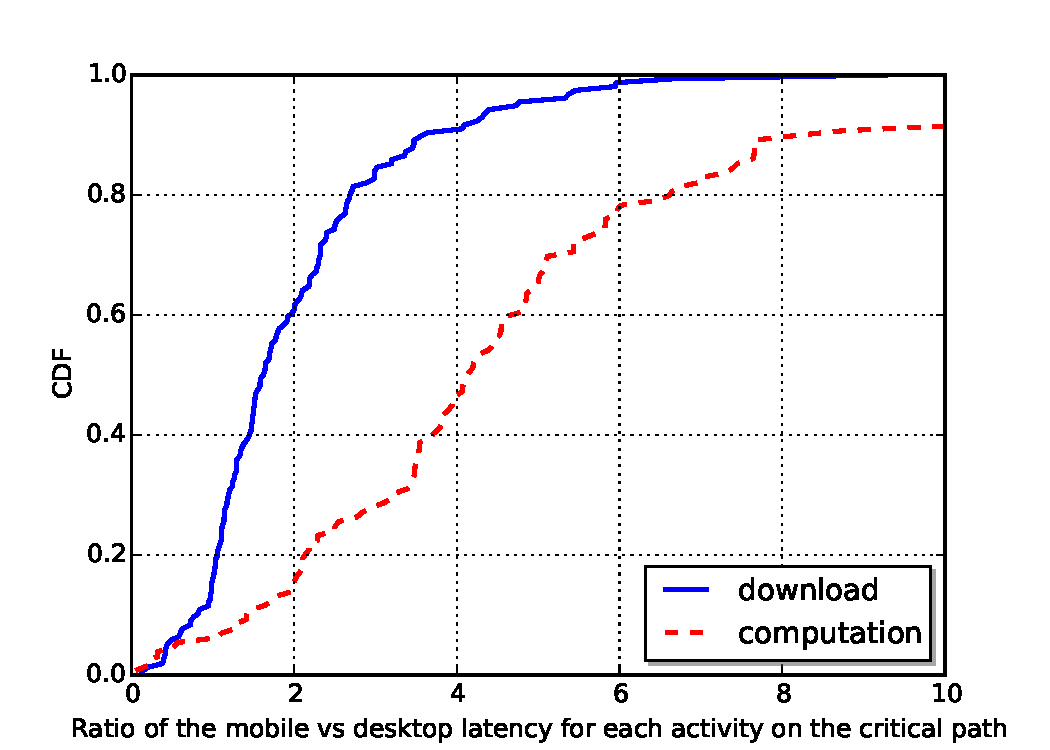
\includegraphics[width=0.5\textwidth]{./figures/criticalpath/latency_comp_network_b20-d50.pdf}
  \caption{Time taken for each activity on the critical path to be performed on the mobile versus desktop browser. Results from loading pages on average lab\_Wifi network. }
  \label{fig:bar_plot_percentage}
\end{figure}




